\documentclass[a4paper,11pt]{article}


% Font
\usepackage[T1]{fontenc}
\usepackage[utf8]{inputenc}
\usepackage{lmodern}
\usepackage{tgbonum} % for extra boldness

% Graphics
\usepackage{graphicx}
\usepackage[usenames,pdftex,dvipsnames]{xcolor}
\usepackage{subcaption}
\usepackage{float}

% Math
\usepackage{amsmath,amssymb,amsthm,textcomp}
\usepackage{enumerate}
\usepackage{multicol}
%\usepackage{tikz}

% Theorem / Proofs
\usepackage{amsthm}
\newtheorem{theorem}{Theorem}
\newtheorem{lemma}{Lemma}
\newtheorem*{remark}{Remark}

\usepackage{geometry}
\geometry{left=25mm,right=25mm,%
bindingoffset=0mm, top=20mm,bottom=20mm}
\linespread{1.3}

%without this package the [H] doesn't run for me (Philip)
\usepackage{float}

%bibliography
\bibliographystyle{unsrt}

% Todo notes
\usepackage{xargs}
\usepackage[colorinlistoftodos,prependcaption,textsize=tiny]{todonotes}
\newcommandx{\unsure}[2][1=]{\todo[linecolor=red,backgroundcolor=red!25,bordercolor=red,#1]{#2}}
\newcommandx{\change}[2][1=]{\todo[linecolor=blue,backgroundcolor=blue!25,bordercolor=blue,#1]{#2}}
\newcommandx{\info}[2][1=]{\todo[linecolor=OliveGreen,backgroundcolor=OliveGreen!25,bordercolor=OliveGreen,#1]{#2}}
\newcommandx{\inlineinfo}[2][1=]{\todo[inline,linecolor=OliveGreen,backgroundcolor=OliveGreen!25,bordercolor=OliveGreen,#1]{#2}}
\newcommandx{\improvement}[2][1=]{\todo[linecolor=Plum,backgroundcolor=Plum!25,bordercolor=Plum,#1]{#2}}
\newcommandx{\thiswillnotshow}[2][1=]{\todo[disable,#1]{#2}}

% my own titles
\makeatletter
\renewcommand{\maketitle}{
  \begin{center}
    \vspace{2ex}
    {\huge \textsc{\@title}}
    \vspace{1ex}
    \\
    \@author \hfill \@date
    \vspace{4ex}
  \end{center}
}
\makeatother
%%%

% custom footers and headers
\usepackage{fancyhdr}
\pagestyle{fancy}
\lhead{}
\chead{}
\rhead{}
\lfoot{GeomLab 2020}
\cfoot{}
\rfoot{Page \thepage}
\renewcommand{\headrulewidth}{0pt}
\renewcommand{\footrulewidth}{0pt}
%

% code listing settings
\usepackage{listings}
\lstset{
  language=Python,
  basicstyle=\ttfamily\small,
  aboveskip={1.0\baselineskip},
  belowskip={1.0\baselineskip},
  columns=fixed,
  extendedchars=true,
  breaklines=true,
  tabsize=4,
  prebreak=\raisebox{0ex}[0ex][0ex]{\ensuremath{\hookleftarrow}},
  frame=lines,
  showtabs=false,
  showspaces=false,
  showstringspaces=false,
  keywordstyle=\color[rgb]{0.627,0.126,0.941},
  commentstyle=\color[rgb]{0.133,0.545,0.133},
  stringstyle=\color[rgb]{01,0,0},
  numbers=left,
  numberstyle=\small,
  stepnumber=1,
  numbersep=10pt,
  captionpos=t,
  escapeinside={\%*}{*)}
}

% No paragraph indentation
\setlength{\parindent}{0in}

% ----------------------
\begin{document}
% ----------------------

\title{GeomLab 2020}
\author{}
\date{\today}
\maketitle

% ----------------------
\tableofcontents
% ----------------------

\newpage

% ----------------------
\section{Motivation}
% ----------------------

In the wake of the COVID-19 pandemic, several outlets printed two-dimensional depictions of data with each symbol representing multiple pieces of information at once. These datasets frequently contained the number of people \textit{infected, recovered} or \textit{dead} due to COVID-19 with regard to the \textit{country} and occasionally the progression of these quantities over \textit{time}.\\

In this lab we will focus on displaying data in meaningful ways. Besides its quantitative nature this task has some qualitative properties. Similar to many solutions of problems in computational geometry, for instance, deciding whether a point is contained in a polygon or the construction of a convex hull for a set of points, the quality of a data plot is obvious to the human observer. Not so for a machine.\\

Consider the two figures shown below. While Fig.\ref{fig:covid2020Feb} is highly informative for humans such as policy makers, Fig.\ref{fig:covid2020May} bears little information content. Both figures, however, were generated by the same depiction algorithm, processing data from the spread of COVID-19 during 2020. The algorithm can be reviewed in the appendix.\\

%
\begin{figure}[h]
  \begin{subfigure}{0.5\textwidth}
    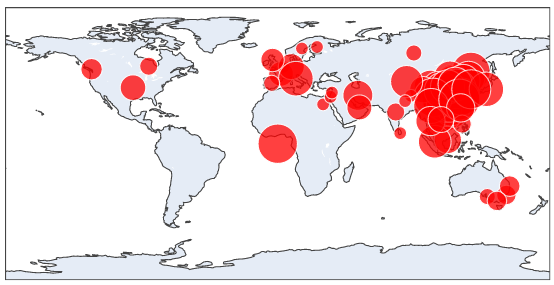
\includegraphics[width=0.9\linewidth]{covid_spread_20200223.png}
    \caption{23.02.2020}\label{fig:covid2020Feb}
  \end{subfigure}
  \begin{subfigure}{0.5\textwidth}
    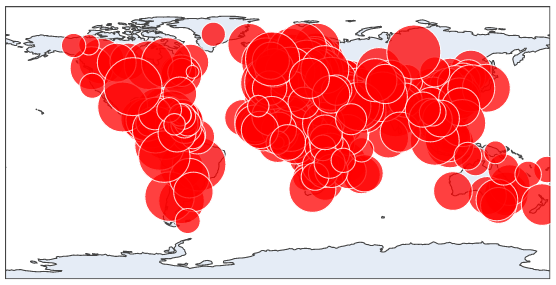
\includegraphics[width=0.9\linewidth]{covid_spread_20200511.png}
    \caption{11.05.2020}\label{fig:covid2020May}
  \end{subfigure}
  \caption{Comparison of a typical scatterplot depicting the $logarithm$ of confirmed cases as the radius.}
  \label{fig:covid19}
\end{figure}
%

For now, we start by defining quantitative measures, i.e. measures of data visibility that can be understood by a computer and assessed on a purely mathematical basis. A discussion on how well the developed algorithms and approaches hold up from a qualitative viewpoint will be conducted later on.\\

Fundamental work into the quantification of visual quality was done both by Tufte in his 1983 book, \textit{The visual display of quantitative information graphics press} and Miller et al. in \textit{The Need For Metrics In Visual Information Analysis}. Based on this, follow-up work and further considerations regarding visibility problems and sorting we develop a novel approach to visualize multidimensional data in a scatterplot designed to transport as much information as possible.\\

Our main resource will be the paper by Sergio Cabello et al. \textit{Algorithmic Aspects of Proportional Symbol Maps}. In it, the authors discuss the difficulty of maximizing utility measures with regards to so-called "physically realizable drawings", in particular they prove this problem to be NP-hard. As a consequence, they restrict their further discussion on a distinct subset of physically realizable drawings, called "stacking drawings" which are determined solely by a total ordering of the symbols, called the "stacking order". They then derive algorithms that determine optimal stacking orders in polynomial runtime. Those algorithms are designed for datasets where each \textit{glyph} only depicts a single quantity.\\

Our goal is to generalize these algorithms so that they may be applied to other types of \textit{glyphs}. We focus in particular on glyphs that visualize multiple quantities, as is needed for data relating to COVID-19, such as nested disks, centered nested disks and pie charts.

\newpage

% ----------------------
\section{Problem Statement}
% ----------------------
Cabello et al. discussed proportional Symbol Maps. Such a map consists of a finite set of $2$-dimensional figures called symbols or glyphs. Each of these glyphs has a position in $\mathbb{R}^2$ and a radius or size corresponding to some quantity given by the data it is supposed to represent. A classic example is the representation of earthquakes and their strength on the Richter-scale. Opaque disks are centered at the epicenter of the earthquake, while the radius corresponds to its strength. In this case, the glyphs are the disks and the associated data encoded in the radius indicates the strength. Other types of glyphs, like squares, hexagons, or pie charts are also possible and are investigated in this lab.\\

The problem is to find a drawing which retains as much of the information about the quantity and the location (center) as possible. More precisely, the raw data alone does not tell you how to deal with overlapping disks, squares or occluded pie pieces. In order to visualize the data on a map we must make several decisions, e.g., one pie occludes a pie segment of a lower pie. Should we change the order? Can we rotate the lower pie such that all of its segments are visible?\\

For the definition of a drawing Cabello et al. describe two approaches, \textit{physically realizable drawings} and \textit{stacking drawings}. For our purposes an intuitive definition of what is talked about will suffice. Those interested in a more detailed definition can consult the original paper \cite{cabello}.\\

Intuitively, a physically realizable drawing can be imagined by taking very flexible glyphs, arranging them in $\mathbb{R}^3$ such that they do not intersect (potentially in a Dali-like fashion) and then taking a picture from a birds eye view.\\
Similarly, a stacking drawing is the same thing but the glyphs are rigid and can only have the same proportions for each point on the same map [TODO: corrected from glyph?].\\

%
\begin{figure}[H]
  \centering
  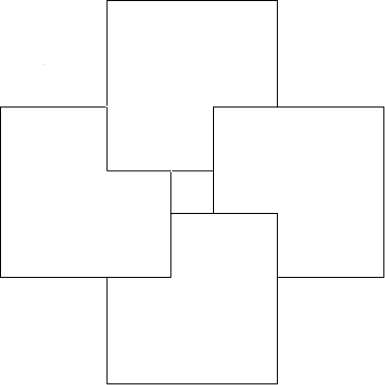
\includegraphics[width=0.4\linewidth]{phys_real_squares.png}
  \caption{A physically realizable drawing of squares which is not a stacking drawing}
  \label{fig:physicalSquares}
\end{figure}
%

Figure \ref{fig:physicalSquares} gives an example of a physically realizable drawing which is not a stacking drawing. The squares overlap cyclically going clockwise "upwards" reminiscent of the "Penrose Stairs". This image can not occur if the squares where embedded with a fixed height as it is required for stacking drawings.\\

A stacking drawing is uniquely determined by the (ascending) order in which the glyphs are stacked on top of one another. This is the so-called \textit{stacking order} of the drawing. Formally, given a finite set $D$ of $n$ glyphs, a stacking order is a bijection $\phi: [n]\rightarrow D$. This bijection describes the order in which the glyphs are drawn. Glyphs which are drawn later may cover parts of the glyphs which are drawn earlier. Therefore our task is to find a stacking order such that as much as possible of every glyph is visible.\\

We are yet to define what we mean when talking about a glyph being as "much visible" as possible. Since this may depend on the type of glyph considered we will turn our attention towards circular disks for now. The other definitions will be delivered as soon as they are needed. We refer to these quantitative measure for the visual quality as \textit{global utility functions}.\\

We take the perspective of an onlooker looking perpendicularly at the map. The viewer should be able to identify the size of the circles and their center points. To achieve this goal, we could try to maximize the visible area of each circle, but there are cases in which that would not allow the viewer to get all of the information. For instance, if the perimeter is not visible at all, then neither the location of the center point nor radius can be determined exactly. The approach we will use is to maximize the visible perimeter of our disks.\\

\newpage

For a fixed stacking order $\phi$, we will denote the disk $\phi(i)$ as $D_i$. We then define the visible and occluded boundary for disks formally by\\
%
\begin{align*}
  U_i^{vis} & =\partial D_i\setminus \bigcup_{j>i} D_{j} \\
  U_i^{occ} & =\partial D_i \cap \bigcup_{j>i} D_{j}.
\end{align*}
%
furthermore, we denote the length of the visible perimeter as $|U^{vis}_i|$. Two global utility functions come to mind:

\begin{align*}
    \lambda_{min} (D) &= \min_{i \in [n]}|U_i^{vis}|\\
    \lambda_{sum} (D) &= \sum_{i=1}^n|U_i^{vis}|
\end{align*}

While $\lambda_{min}$ is focused on the least visible perimeter, $\lambda_{sum}$ sums up the visible length of all perimeters. Key results proven in \textit{Algorithmic Aspects of Proportional Symbol Maps} are the following
\begin{theorem}
  It is NP-hard to decide if a given collection of congruent disks has a
  physically realizable drawing where at least some given length of the perimeter of
  each disk is visible.\qed
\end{theorem}
This implies that trying to maximize the minimal $|U_i^{vis}|$ with respect to physically realizable drawings is NP-hard.
\begin{theorem}
  It is NP-hard to decide if a given collection of disks has a physically
  realizable drawing whose total visible perimeter is at least a given value.\qed
\end{theorem}
This implies that trying to maximize the sum over all the $|U_i^{vis}|$ with respect to physically realizable drawings is NP-hard.\\
For stacking orders the objective returns a positive result with regards to the minimum:
\begin{theorem}
  Given n disks in the plane, a stacking order maximizing the boundary
  length of the disk that is least visible can be computed in $O(n^2 \log n)$ time.\qed
\end{theorem}
Whether a polynomial algorithm for the sum of all visible perimeters exists remains an open question.\\


\newpage

We won't attempt to construct an algorithm for the sum problem and instead take a look at glyphs which are able to depict more than one piece of information.\\

The first type of glyph we discuss are nested disks. Formally, every glyph $G^i$ is given by a set of disks $G^i_1,...,G^i_k$ such that $G^i_{j+1}\subset G^i_j$ for all $j\in \{1,...,k-1 \}$. Often times figures using nested disks also center all the disks at the same point.\\
The second type of glyphs we use are pie charts. A pie chart is formally given by a disk $D_i$ and a set $\{\alpha_1^i,...\alpha_k^i\}$ of dividing lines which we can encode as angle in $[0,\ 2\pi]$. Usually the dividing lines separate areas of different color representing different fractions of a sum.\\

In the next section we will discuss a simple and versatile approach to determine optimal stacking orders for glyphs maximizing utility functions with specific properties for glyph stacking order drawings and then apply it to our glyphs and some utility functions.

% ----------------------
\section{Stacking order algorithms for more general Glyphs}
% ----------------------

The function $\lambda_{min}$ from above provides an example of a global utility function for which an optimal stacking order can be computed via a simple greedy algorithm. At each time step just calculate for all disks their visible perimeter as if they were the bottommost disk, choose the disk $D_i$ with the largest visible perimeter and put it on the bottom. In the next time step we look at the set of disks without $D_i$ and repeat the procedure. This is done until we have processed all disks.\\

We can now formalize this approach for more general objects and prove that the greedy algorithm is optimal with respect to the utility.\\

Let $D$ be a finite set and for $d \in D$ and $S \subseteq D$ the function $ \Gamma(d, S) \mapsto \mathbb{R}_{\geq 0} $ with the property, that for every $d \in D$ we have $S' \subseteq S \implies \Gamma(d, S') \geq \Gamma(d, S)$. \\

The set $D$ corresponds to our set of glyphs and $\Gamma$ corresponds to a local utility function, which depends on the insertion order, i.e, the set $S$ is thought of as the set of all glyphs which lie above $d$. Let $\phi: \{1,...,n\} \mapsto D$ be a stacking order. Then for every glyph $d_i:=\phi(i)$ the set of glyphs above $d_i$ is given by $\{d_j\in D\ |\ j > i\}$.

\begin{figure}[H]
  \begin{lstlisting}[mathescape=true]
GreedyStacking(finite set $D$)
  $x := \text{argmax}_{d \in D} \Gamma(d, D \setminus {d})$
  return [$x$, ALG($D \setminus {x}$)]
  \end{lstlisting}
  \caption{The greedy stacking algorithm}
  \label{fig:greedyalg}
\end{figure}

\newpage

\begin{theorem}
  For a given set $D$ and a local utility function $\Gamma$ the greedy algorithm as described in \ref{fig:greedyalg} returns a stacking order $s$ which maximizes
  \begin{align*}
    \lambda(s) = \min_{i \in \{1,\dots,n\}} \Gamma(s(i), \{s(j)\ | j > i\}).
  \end{align*}
\end{theorem}

\begin{proof}
To prove the above theorem we define $s^*$ the stacking order generated by the algorithm. We will then prove that for any other order $s\neq s^*$ that there is a modified order $s'$ that fulfills $\lambda(s)\leq\lambda(s')$ and that overlaps with $s^*$ in at least one more additional spot.

Consider $s\neq s^*$ and let $i=\min\{l\ |\ s(l)\neq s^*(l)\}$ the first index for which $s$ and $s^*$ disagree. The glyph $s^*(i)$ has a different index according to $s$, namely, the index is $j=s^{-1}(s^*(i))$ and, because $i$ is the minimal index of disagreement, we have $j>i$.

We modify $s$ as follows. Instead of choosing glyph $s^*(i)$ only in index $j$, the new stacking order $s'$ selects it at $i$ as well and increases the index of $s(l)$ by $1$ for $l\in [i,...,j-1]$. More formally, $s'=s\circ \tau$, where

\[
\tau(k) = \left\{\begin{array}{ll}
    k-1, & \text{for } k\in [i+1,\dots,j]\\
    j, & \text{for } k=i\\
    k, & \text{else}\\
    \end{array}\right\}
\]

Clearly, $s'(i) = s\circ\tau(i) = s(j) = s^*(j)$ and for $k<i$, $s'(k) = s\circ\tau(k) = s(k) = s^*(k)$, so $s'$ disagrees with $s^*$ only at a later stage. We claim that $s'$ is as least as good of a solution as $s$, meaning $\lambda(s')\geq\lambda(s)$. If this holds true we can, by iterative application of the previous modification, construct for any stacking order $s$ a non-decreasing sequence $s, s', s'', \dots, s^*$ ending in $s^*$, the stacking order generated by the algorithm. Thereby proving that $s^*$ is optimal.

The proof of the claim rests on the following observation: Recall that the $\Gamma$-value is anti-monotonous, meaning its value increases as the second argument decreases. All the objects that either maintain the same index or get it increased by one only have a subset of glyphs above them as compared to before the modification, meaning their values increase. Only the glyph whose index changes from $j$ to $i$ has a growing set of glyphs above it. However, this object is selected by the algorithm at index $i$ so it has to be at least as good as the glyph selected by $s$. Thus, the utility of each disk as arranged in $s'$ is bounded below by the utility of some disk as arranged in $s$.

To make this formal, we prove the following:

\begin{equation}
    \forall k'\in[n]\ \exists k\in[n]:\ \Gamma(s'(k')|\{s'(l), l>k'\})\geq\Gamma(s(k)|\{s(l), l>k\})
\end{equation}

Consider first $k'\notin \{i,\dots,j\}$, then
\[\Gamma(s(k'),\{s(l),\ l>k'\}) = \Gamma(s'(k'),\{s'(l),\ l>k'\})\]
because both $s(k')=s'(k')$ and $\{s(l),\ l>k'\}=\{s'(l),\ l>k'\}$. We can choose $k=k'$.

If $k'\in [i+1,\dots,j]$, then
\[ \Gamma(s'(k'),\{s'(l),\ l>k'\}) \geq \Gamma(s'(k'),\{s(l),\ l>k'-1\}) = \Gamma(s(k'-1),\{s(l),\ l>k'-1\})\]

where the inequality comes from the second argument on the left-hand side being a subset of the one on the right, so $k=k'-1$ and lastly for $k'=i$

\begin{equation*}
\begin{split}
\Gamma(s'(k'),\{s'(l), l>k'\}) &= \Gamma(s'(i),\{s'(l),\ l>i\})\\
&=\Gamma(s^*(i),\{s^*(l),\ l>i\})\geq\Gamma(s(i),\{s(l),\ l>i\})
\end{split}
\end{equation*}

Here, the first equality is simply substituting $k'=i$. The second one comes from $s'$ and $s^*$ agreeing for $l\leq i$ and the inequality holds because $s^*(i)$ is the choice of the algorithm and thus maximizes precisely this term, so $k=i=k'$ does the job.

In total

\begin{equation*}
\begin{split}
    \lambda(s') &=  \min_{i \in \{1,\dots,n\}} \Gamma(s'(i), \{s'(j)\ | j > i\})\\
    &= \Gamma(s'(k'), \{s'(j)\ |\ j > k'\}) \text{ for some }k'\\
    &\geq^{(1)} \Gamma(s(k), \{s(j)|\ j>k \}) \text{ for the corresponding }k\\
    &\geq \min_{i \in \{1,\dots,n\}} \Gamma(s(i), \{s(j)\ | j > i\}) = \lambda(s)
\end{split}
\end{equation*}

proving that $s'$ is as least as good a solution as $s$.
\end{proof}

We can use this theorem for glyphs of any kind. In particular for the glyphs we discussed before so long as the utility function can be modelled as described in the theorem.\\

With this, the crux is to define meaningful utility functions for different glyphs and evaluate them locally with feasible runtime.

\subsection{Centered nested disks}

For centered nested disks we can easily define local utility measures. Every glyph $G$ corresponds to $k$ nested circles therefore we could just calculate the visible perimeter for the $k$ circles and then just combine them by choosing the minimum of the $k$ circles or the sum of the visible perimeter of the $k$ circles. For some set $S$ of objects above $G_i$ we then get formally:

\begin{align*}
  \Gamma_{min}({G^i,S})=\min_j  {^{vis} G^i_j} \\
  \Gamma_{sum}({G^i,S})=\sum_{j=1}^k  {^{vis} G^i_j}
\end{align*}

We may also be interested in the relative utility which is derived for a glyph by only taking the visible percentage of each nested circle into consideration. This relative approach stops the small circles from dominating big circles. In our applications there is close to no difference between the relative and absolute utility.\\

For $\Gamma_{min}$ it may happen that for all glyphs the smallest circle may be completely covered. Then the utility would be zero for all of the circles. If this happens the algorithm has an optimal solution of value zero. In case of this situation, we follow the heuristic to perform the greedy step again and ignore the smallest circle in all of the glyphs until we get a value bigger than zero. This heuristic gives better results than just choosing a random circle, since it guarantees that at least in this time step the least amount of circles get covered.\\
%
\begin{remark}
It is NP-hard to calculate physically realizable drawing where $\min\Gamma_{min}$ or $\min\Gamma_{sum}$ is maximized since disk glyphs are a special case of nested disks and both utility measures coincide and are equal to the visible circumference.
\end{remark}
We are primarily interested in the quality of the optimization, not the runtime of the computing algorithms. Therefore we use a naive implementation to calculate the stacking with runtime $O(n^3k^2)$. The runtime could be improved to $O(n^2k \log nk)$ by adapting the data structure introduced in \cite{cabello}.


% ----------------------
\subsection{Nested disks}
% ----------------------

For dense regions, centered nested disks lose a lot of information since the small circles can be completely covered up easily. Therefore, we will now derive an algorithm which guarantees that every nested circle is at least visible. To achieve that we will allow the circles to be moved within each other. We still want to have $G^i_{j+1}\subset G^i_j$ for all $j$, however, now the centers don't have to coincide.\\

Our approach is straightforward. We first just look at the biggest circle of each glyph. For those we perform our greedy algorithm with the local utility given by the size of the maximal \textit{continuous} visible perimeter. After we have done that we can take the point $p$ on the circle which is in the middle of the longest continuous perimeter piece visible and connect it to the center of the big circle by a line. Now every center point for a nested inner circle is uniquely defined by positioning it on that line such that the circle touches the point $p$. The final glyphs look a little bit like the \textit{Hawaiian earring} topological space.\\

The resulting drawing guarantees that the perimeter of every circle is at least a little bit visible. The downside of this construction is that the drawing look a little bit strange to the viewer and its more difficult to identify the center of a glyph.\\

We again use the naive approach for disks from \cite{cabello} with runtime $O(n^3)$. Since we are only interested in the largest disk the number of nestings $k$ only adds a linear term. Therefore the overall runtime is given by $O(n^3+nk)$. As described in \cite{cabello} the runtime could be improved to $O(nk+n^2 \log n)$.


% ----------------------
\subsection{Pie charts}
% ----------------------

Recall a pie chart glyph is given by a disk $D_i$ and dividing lines given by a finite set $P_i= \{\alpha_1^i,...\alpha_m^i\}$. The $\alpha_j$ are given by angles in $[0,2\pi ]$. We may rotate the dividing lines like minute or hour hands on a mechanical watch. However, the relative distance between all angles must stay the same. Hence, a rotation can be described by a single angle due to the fixed relative distance of the dividing lines. Given a rotation of the angles and a set $S$ of glyphs which lie above the pie chart in our drawing we can define $\Gamma_{pie}(D_i,S)$ as the minimal radial distance of any of the $\alpha^i_j$ to the covered perimeter. If the perimeter is completely visible, then this distance is defined by half the circumference or $\pi r_i$.\\

Now we need to investigate two things:

\begin{enumerate}
  \item Is it feasible to optimize the aforementioned utility function with respect to physically realizable drawings generally or do we need to restrict ourselves to stacking drawings? The pie chart glyphs are not a natural generalization of the disks. Therefore we cannot argue NP-hardness as easily as in the case of nested disks.
  \item In addition to deciding which pie covers which we also have to specify a rotation for each pie. How do we calculate the optimal rotation for a given pie knowing which pies lie above it?
\end{enumerate}

% ---
\subsubsection{NP-hardness}
% ---

\subsubsection*{Setting}
Given a finite set $D$ of disks $d_i$ in the plane with centers $c_i$ and positive radii $r_i$ together with a finite set $P_i = \{ \alpha_1, \dots, \alpha_{m_i}\}$ of points on the boundary of $d_i$ subdividing the disk into pie-pieces we wish to determine a physically realizable drawing of $D$ together with a rotation $\varphi_i$ for each disk such that the minimum distance of any point in $p\in\bigcup P_i$ to the next occluded point on the boundary of $d_i$ is maximized.
I.e., we are given Pie-Charts and would like to arrange and rotate them in such a manner that the points where the transition-lines of the pie-chart meet the boundary are as far from being occluded as possible. [TODO: I don't get this sentence]

\subsubsection*{Theorem}
It is NP-hard to decide, whether for a given set $D$ of disks with boundary points $P_i$ there is a physical realization (with rotation) such that the minimum distance of any of the distinguished points $p_i$ to the next occluded point along the perimeter of its perimeter is greater or equal to $k$. Or formulated as formula:

\[\min_{i\in [n]} \Gamma(D_i,\{D_j\ |\ j>i\}) \geq k\].

\subsubsection*{Proof}
The proof is inspired by and in large parts analogous to the proof of Theorem 1 \cite{cabello}.
We aim to reduce the NP-hardness from $planar$-3-SAT, i.e., instances $\mathcal{I}$ of 3-SAT with the property that the graph $G(\mathcal{I})$ is planar.
The graph $G(\mathcal{I})$ is bipartite, has a node for each variable on one side and each clause on the other. A variable node is connected to the clause iff one of it's literals appears in the clause.\\

\textbf{Example:}
\[ \mathcal{I} = \underbrace{(x_1 \vee x_2 \vee \overline{x_3})}_{C_1} \wedge \underbrace{(x_3 \vee \overline{x_4} \vee x_5)}_{C_2} \]

\begin{figure}[h]
\centering
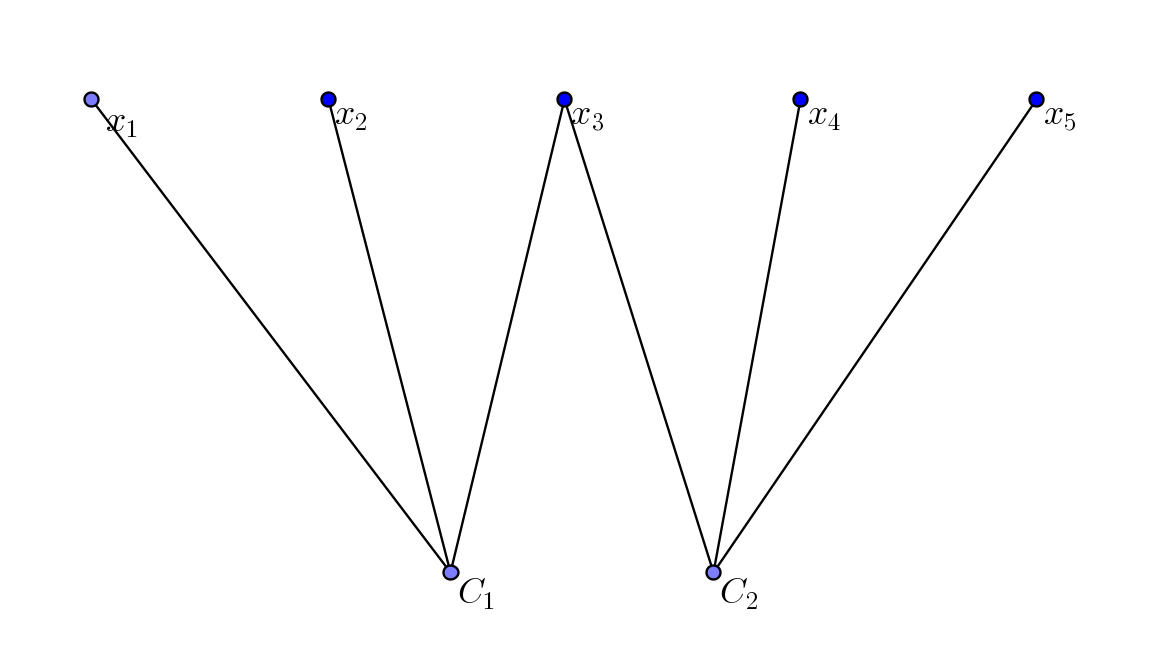
\includegraphics[width=15cm, height=10cm]{assets/np-hardness/incidence_graph.png}
\caption{The incidence graph $G(\mathcal{I})$}
\end{figure}

Given a planar instance $\mathcal{I}$ of 3-SAT we need to construct an instance $\mathcal{D}$ of our pie-charts such that $\mathcal{I}$ is satisfiable iff $\mathcal{D}$ has a physical realization with distance $\geq k$ for some suitable $k$.

All the disks presented have the same radius and we say that two disks overlap by $f$ if the overlapped fraction of the boundary has length $f$. We introduce the construction of $\mathcal{D}$.

\subsubsection*{Construction}
\begin{figure}[h]
\centering
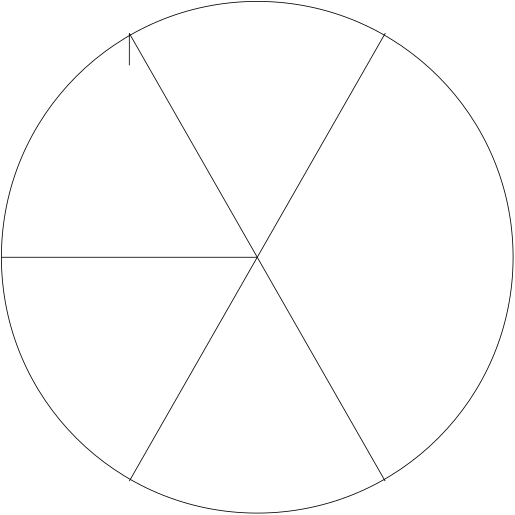
\includegraphics[width=5cm, height=5cm]{assets/np-hardness/neutral.png}
\caption{A "neutral" disk used as a connector within a variable ring. The angles are 60 and 120 degrees}
\label{fig:neutral}
\end{figure}

\begin{figure}[h]
\centering
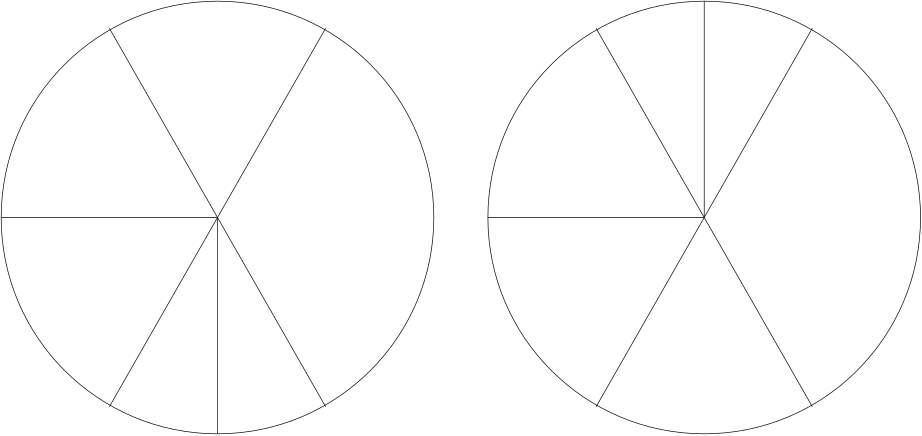
\includegraphics[width=10cm, height=5cm]{assets/np-hardness/true_false.png}
\caption{A "true" and "false" disk, similar to the neutral one above, one of the 60 degree segments is cut in half}
\label{fig:trueandfalse}
\end{figure}

We use the three disk types in Figures \ref{fig:neutral} and \ref{fig:trueandfalse} to construct for each variable in the 3-SAT instance a so-called "gadget". A gadget is a group of neutral disks forming an elongated band each overlapping the next by a fraction of 1/4 or 90 degrees. Notice that the maximum possible distance of separation points to occluded area is 15 degrees, because the segment is covered at 120 degrees and 90. The gadget is constructed in such a way that it can only be oriented clockwise or counter-clockwise if we want $k>0$ separation between the lines to the occluded area.

Figure \ref{fig:gadget} depicts a prototype of a gadget: All the disks are of the neutral type for now. The curvature is created by connecting the disks at a 45 degree angle while still overlapping by a fraction of 1/4.

\begin{figure}[H]
\centering
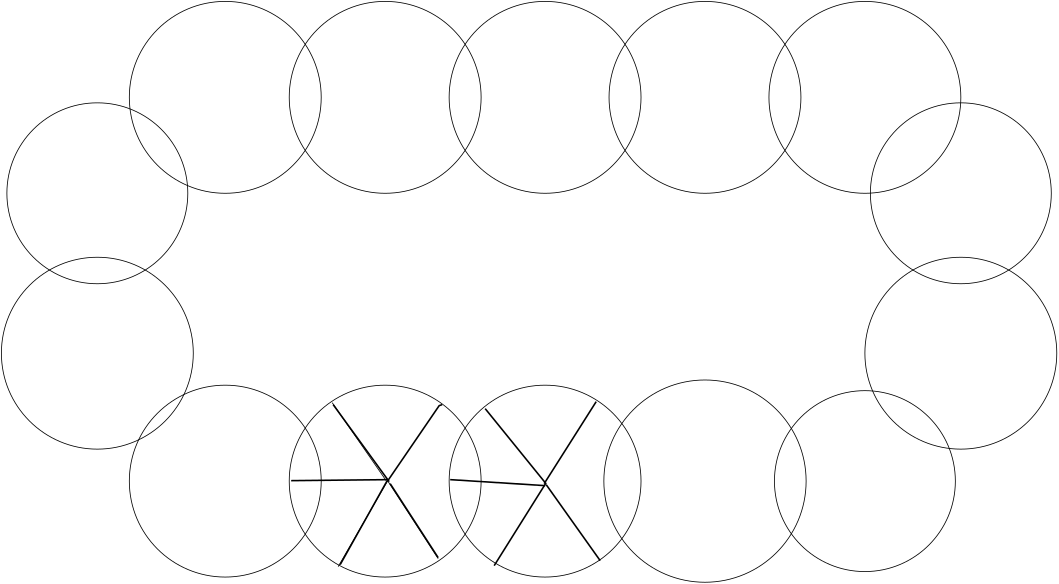
\includegraphics[width=10cm, height=5cm]{assets/np-hardness/gadget.png}
\caption{One such gadget $G_i$ for each variable $x_i$}
\label{fig:gadget}
\end{figure}

We will interpret a gadget in ascending clockwise order as the corresponding variable being "true" and otherwise "false". [TODO: What is the second half of the sentence about?]

For each occurrence of the variable $x_i$ in any of the clauses we will substitute a neutral disk in the gadget $G_i$ by either a "true" or "false" disk as depicted in Figure \ref{fig:trueandfalse}. We use a "false" disk if the literal appears negated in the clause.

\begin{figure}[h]
\centering
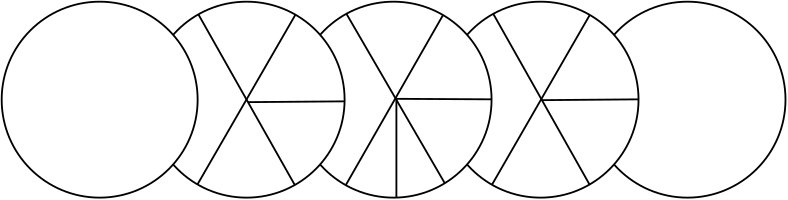
\includegraphics[width=15cm, height=4cm]{assets/np-hardness/negative.png}
\caption{A segment of a "true" gadget with a "false" disk in it}
\end{figure}

The above segment is of a "true" gadget as the disks are clockwise ascending. The "false" and "true" disks will ensure that the added segment will point outwards iff the corresponding literal in the clause is false.

Next we will focus on how the clauses will be set up. Later we will connect the gadgets and the clauses, which is why we require the instance to be planar.

\begin{figure}[H]
\centering
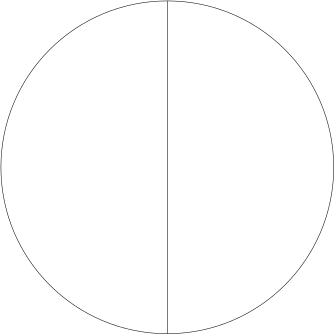
\includegraphics[width=5cm, height=5cm]{assets/np-hardness/clause.png}
\caption{One such disk for each clause}
\end{figure}

Recall that the instance is satisfiable iff each clause is fulfilled. We instantiate one disk as above for each clause. It has two separating lines exactly opposing one another. For each literal in the clause we overlap it with one of the disks shown below by a fraction of 1/4 as shown in Figure \ref{fig:clauseconnection}. [TODO: This sentence is confusing.]

\begin{figure}[h]
\centering
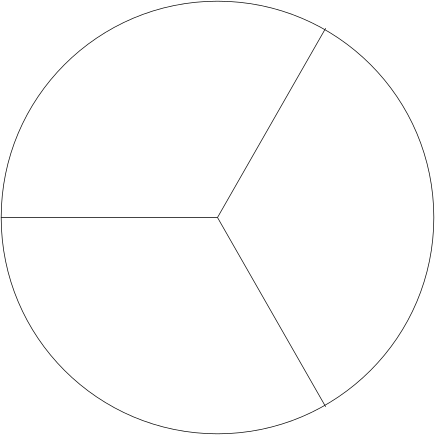
\includegraphics[width=5cm, height=5cm]{assets/np-hardness/clause_connector.png}
\caption{This disk is the endpoint of the edge connecting the gadget to the clause disk}
\end{figure}

This connector disk is supposed to be above the clause-disk iff its associated literally as is "false" in the clause. [TODO: This sentence is confusing.]

\begin{figure}[h]
\centering
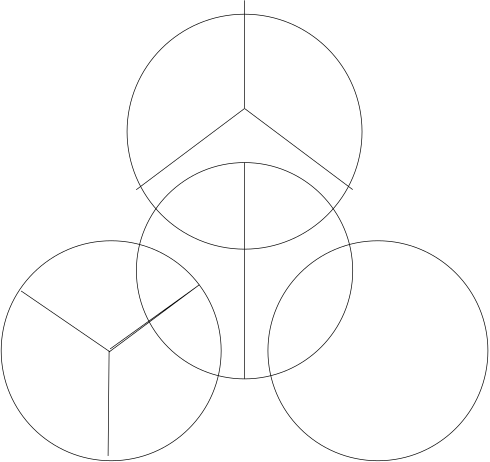
\includegraphics[width=5cm, height=5cm]{assets/np-hardness/literal_clause.png}
\caption{The clause together with the literal connectors}
\label{fig:clauseconnection}
\end{figure}

The clause disk is overlapped by three connector disks each overlapping 90 degrees and leaving three 30 degree corridors. If the upper connector disk can be rotated as depicted then it may go under the clause disk, signifying the literal is "true" in the clause. Otherwise it must go over, like the bottom left one. [TODO: And what does this mean? "false"?]
If all three connectors go over the clause, then the clause disk cannot have 15 degrees of space between the separating points and the occluded area. If, conversely, at least one of them goes under, like potentially the top one in Figure \ref{fig:clauseconnection} then by rotating the clause disk as depicted creates 15 degrees of length between the lines and the occluded area.

Now we need to bring it all together. Recall that we have gadgets that can be oriented clockwise or counterclockwise to signify a "true" or "false" assignment of the variable. The gadgets have for each variable-clause pair a special "true" or "false" disk that will point a separating line outwards iff the $literal$ is false in the clause. We also have connectors at the clause that will act as if "false" iff they go over the clause disk, which has to occur if their separating line cannot be arranged as in the top disk of Figure \ref{fig:clauseconnection}.

What we need to ensure is that the connector disk cannot be rotated like that if the literal disk in the gadget points outwards. To do this we introduce the last building block of the construction.

[TODO: RS stopped reading here for now]

\begin{figure}[h]
\centering
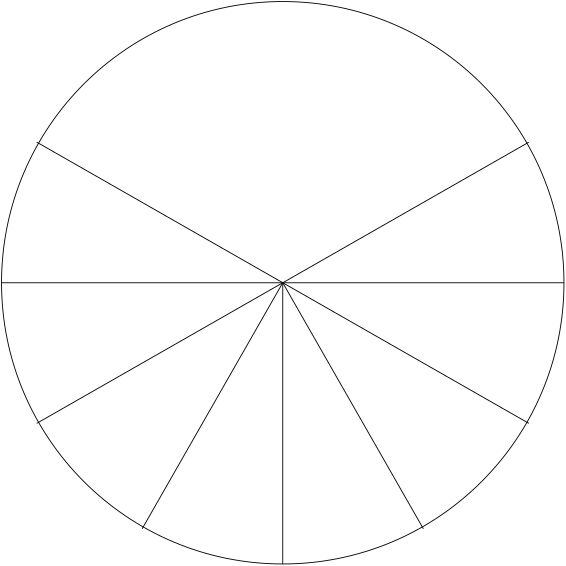
\includegraphics[width=5cm, height=5cm]{assets/np-hardness/literal_connector.png}
\caption{These disks connect the gadgets to the corresponding clauses}
\end{figure}

These disks will be arranged in a line connecting the "true"/"false" disks in the gadget with the clause-connector disks at the clause like so:

\begin{figure}[h]
\centering
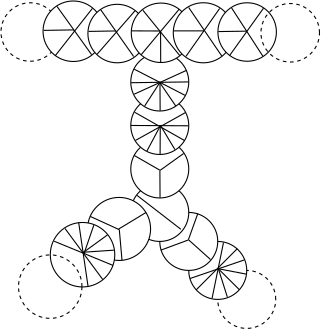
\includegraphics[width=10cm, height=10cm]{assets/np-hardness/full.png}
\caption{These disks connect the gadgets to the corresponding clauses}
\end{figure}

The top gadget is oriented as "false" and the "true" disk in the middle thus has a separator pointing outward. This forces the first outgoing connector, which overlaps the "true" disk by 1/12 = 30 degrees to be under it and point its own separators downwards as well. This continues until the clause-connector disk is reached which now cannot be oriented as the bottom-right own and has to go over the clause-disk.

\subsubsection*{Example}
Example will be depicted here.

\subsubsection*{Conclusion}
The logical properties were already explained when motivating the construction but will be formalized here again. Notice that the disks in the clause and the gadget can create a distance of 15 degrees between occlusion and separation points. We claim the following.
Given a planar instance of 3-SAT $\mathcal{I}$ and the corresponding construction $\mathcal{D}$ as above, $\mathcal{I}$ is satisfiable if and only if there is a physical realization of $\mathcal{D}$ that creates a distance of at least 15 degrees $=(15/360\cdot 2\pi)$.

Given a satisfiable instance we orient the gadgets according to the assignment. This will make all "false" connections point a separator outward. Within the gadgets, all disks maintain a distance of at least 15 degrees to the other disks in the gadget. The connector disks at these "false" connections will have to go under so that the outpointing separator has distance $\geq 0$, let alone 15. The "true" connections are not forcing the outgoing connections to go under, we will place them above giving a distance of exactly 15 degrees. This connection line will be going "upwards" (as viewed from gadget to clause) until it reaches the clause connector, which now can be placed under the clause-disk enabling it to also create a distance of at least 15 degrees.
This implies that all disks can create a distances of 15 degrees to their occluded boundary segments.

Conversely, if the constructed instance has a physical realization with degrees $\geq 15$, then clearly in each clause-disk we must have a least one of the connector going below it. This is only possible with distance $\geq 15$ if the separators are directed away from the clause disk and thus forcing the rest of the connection to go "upwards" (as viewed from clause to gadget). This means that the first disk in the gadget must be under the last disk in the connecting line. This is only possible if the literal is "true" meaning the variable is "false" and the literal negated or "true" and the literal in normal form. We obtain and orientation of the gadgets that is consistent with all clauses and thus a satisfying assignment of the variables in $\mathcal{I}$.\qedsymbol

% ---
\subsubsection{Optimal rotations for $\Gamma_{pie}$}
% ---

Given a set $S$ of covering glyphs and a fixed pie chart $C_i$ we can calculate the occluded radial intervals $I_1,...,I_k$ on the boundary circle of $C_i$. We now want to find a rotation of the dividing lines that maximizes the minimal distance of any of the $\alpha^i_j$ to the occluded intervals. We can look at this rotation with respect to some reference line. Here we use $\alpha_1$ as the reference line.\\

Now we want to derive all of the positions on the circle where the reference line can be positioned such that none of the dividing lines are covered on the boundary. We will derive the complementary intervals first, i.e., all the intervals that guarantee that at least one dividing line is occluded.

\begin{lemma}
  Given a set of occluded intervals $I=\{[a_1,b_1],...[a_k,b_k]\}$ (as angles) and a set of dividing lines $\{\alpha_1,...\alpha_m\}$ also given by angles, let $\beta_j$ be the counterclockwise angular distance from $\alpha_1$ to $\alpha_j$ for $j\in\{1,\dots,m\}$, and let $\mathcal{I}$ be the set system given by
  \begin{align*}
    \mathcal{I}=\bigcup_{i=1}^m    \bigcup_{j=1}^k \{ [a_j-\beta_i,b_j-\beta_i]   \}.
  \end{align*}
  Then any rotation which locates $\alpha_1$ in one of the intervals in $\mathcal{I}$ occludes at least one dividing line. Conversely, any rotation locating $\alpha_1$ in none of the intervals in $\mathcal{I}$ will occlude none of the lines.
\end{lemma}

\begin{proof}
    "$\implies$": Consider a rotation $\beta$, s.t. $\alpha_1 + \beta \in \mathcal{I}$, then $\alpha_1 + \beta \in [a_j - \beta_i, b_j-\beta_i]$ for some pair $(i,j)$. Note that $\alpha_1 + \beta_i = \alpha_i \implies \alpha_1 = \alpha_i - \beta_i$. Therefore, $\alpha_i-\beta_i+\beta\in[a_j-\beta_i, b_j-\beta_i]$ and thus $\alpha_i+\beta\in[a_j, b_j]$. The line represented by $\alpha_i$ will be occluded.\\
    "$\impliedby$": Analogously.
\end{proof}

The complement of $\mathcal{I}$ on the circle describes all of the locations of $\alpha_1$ which do not occlude any dividing line. This complement may be empty since there may not be a rotation which does not occlude any line. With this observations we now can easily derive an algorithm which returns a rotation which maximizes our utility.

\begin{theorem}
  Given a set of occluded intervals $I=\{[a_1,b_1],...[a_k,b_k]\}$ (as angles) and a set of dividing lines $\{\alpha_1,...\alpha_m\}$ also given by angles, Algorithm 2 returns a rotation which maximizes the minimal radial distance of any of the $\alpha^i_j$ to the covered perimeter.
\end{theorem}
% TODO: Labels (after everything else is nice probably)

\begin{proof}
  Algorithm 2 rotates a given dividing line in such a way, that it lies exactly in the midpoint of the biggest not occluded interval $[a_v, b_v]$. The midpoint in an interval is the point which has the maximum distance from both boundaries, $a_v$ and $b_v$. As the biggest not occluded interval maps to the circle's perimeter, it also maximizes the distance to the boundaries of the occluded intervals $\{[a_1, b_1], ..., [a_k, b_k]\}$.
\end{proof}

\begin{figure}[!bth]
  \begin{lstlisting}[mathescape=true ]
Input: $I=\{[a_1,b_1],...[a_k,b_k]\}$ $\{\alpha_1,...\alpha_m\}$)
  calculate $\mathcal{I}=I \cup \bigcup_{i=2}^m    \bigcup_{j=1}^k \{ [a_j-\beta_i,b_j-\beta_i]   \}$
  let $\mathcal{V}$ be the set of maximal continuous intervals in $[0, 2\pi]\setminus {\mathcal{I}}$
  $v=[a_v,b_v]$ biggest interval in $\mathcal{V}$
  $r=(b_v+a_v)/2$
  return r
  \end{lstlisting}
  \caption{IntervalMidpointAlgorithm}
\end{figure}

With this algorithm we can again use our general greedy algorithm for stacking orders.\\

If we use a naive implementation for Theorem 5 we get a runtime of $O(n^3k^2)$. Again the data structure introduced in \cite{cabello} could be used for the pie glyphs which yields a runtime of $O(n^2k \log nk)$. This adaptation would need some work, since the pie glyphs are not immediately  compatible with the data structure.\\


It may happen again that for all glyphs the local utility is zero. Again we have to use a heuristic to get better results. For instance, we can just ignore one dividing line for each glyphs and try again. This can be done iteratively until the utility is not zero for all glyphs. For the case of exactly one dividing line the utility must be bigger than zero and therefore the heuristic guarantees a better decision than just randomly tie breaking.

\subsection{Squares}
The last glyph we discuss are squares which are subdivided into smaller rectangles. We don't restrict ourself to axis aligned squares. Therefore the algorithms we discuss may rotate the squares to get better results with respect to the visibility.\\
Cabello et al. only discussed axis aligned Squares in \cite{cabello}. There hasn't been any theoretical discussion with regards to rotatable squares and visibility as far as we know. Our greedy stacking theorem would not apply to  rotatable squares since the local utilities may only depend on the order, but the rotation we perform at time step $t$ could change some of the local utilities for squares which have been drawn before time $t$.\\
For that reason we would need some new approach to get any optimal results and it may even be NP-hard to calculate a stacking with optimal rotations with respect to the visibility of the perimeter of the squares.\\

Our main focus in this Lab was the visualisation of multiple features, e.g. in the case of covid-19 infected,dead and recovered. Consequently we do not try to derive optimal algorithms for the single feature case and just recycle some of our other results to get a heuristic solution for our problem with respect to squares.\\
We now derive a data representation in the form of squares and sub-rectangles for exactly $3$ features. Our glyph will be given by a Square $S$, such that the length of the sides represents the sum of the features with respect to some scaling. Then we insert an orthogonal dividing line $l_1$ which divides the square into two rectangles such that one of the rectangles $r_1$ contains an area proportional to the largest feature. With a second line $l_2$ the other rectangle is divided into to rectangles $r_2$ and $r_3$ which each contain an area proportional to the other features. See Figure 15 for an example of such a glyph.\\
\begin{figure}[b]
\centering
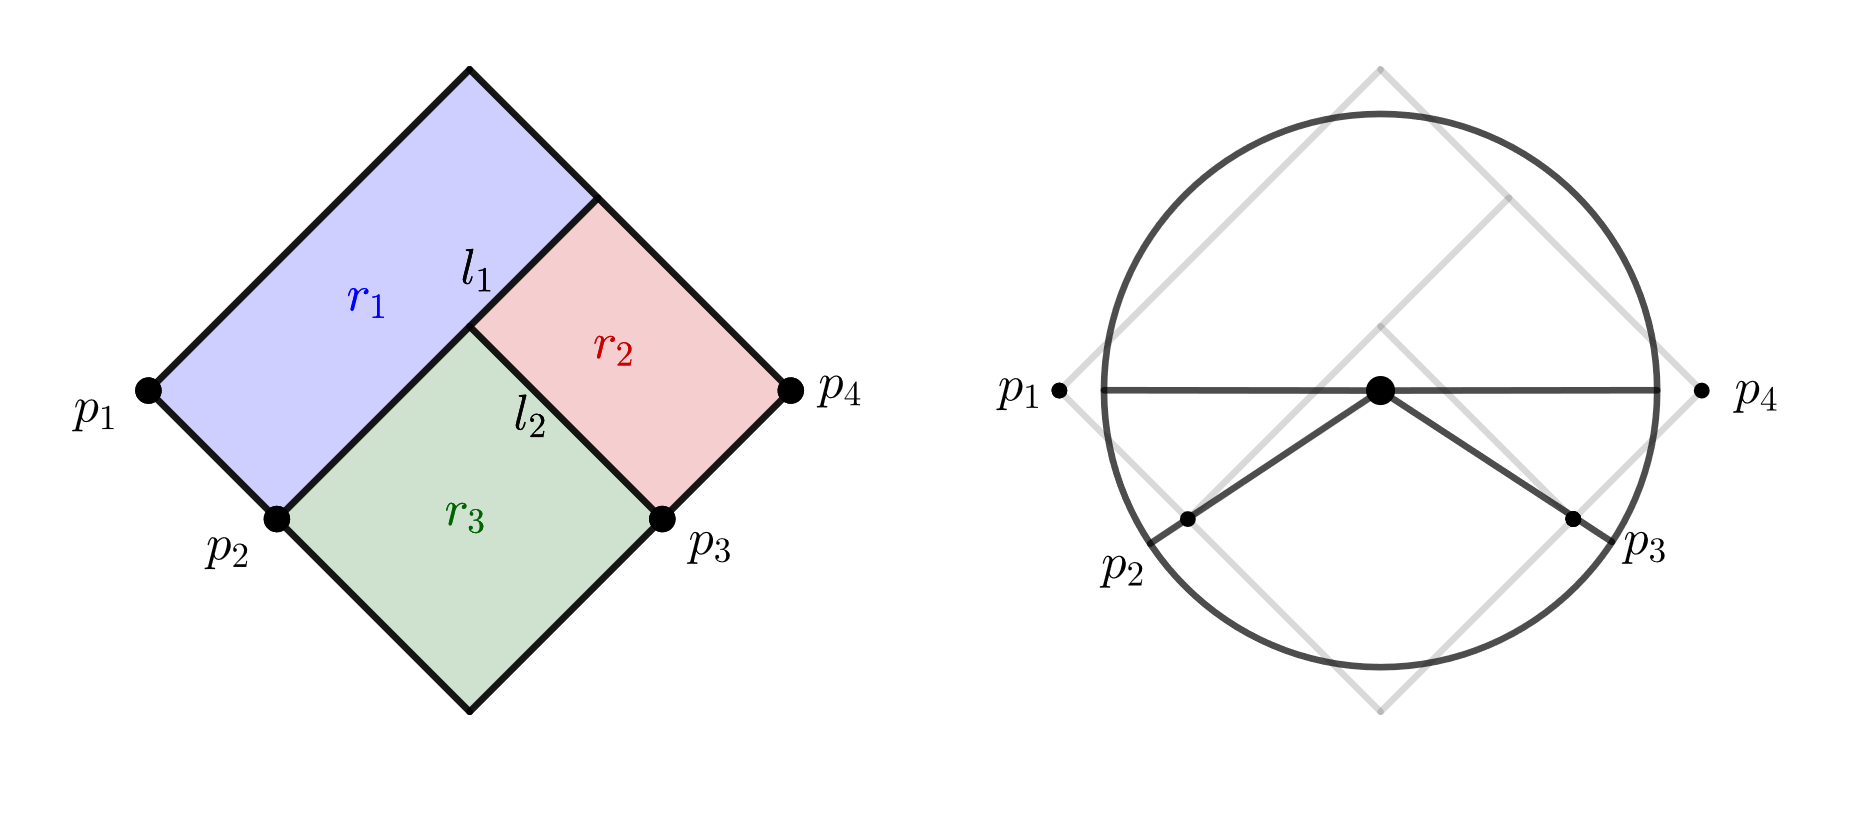
\includegraphics[height=4cm]{assets/square_glyphs}
\caption{left:square glyph, right: heuristic pie chart}
\end{figure}

In order to guarantee that the user can get all of the depicted information, he needs to see to diagonal corner points of the square and one point on the border for each line. We chose the point $p_1,p_2,p_3$ and $p_4$ which are displayed in Figure 15 for our algorithm. The local utility of a square would be the minimal distance of the points to the occluded perimeter.\\
We can get a good solution with the help of pie charts. For every square we construct a pie chart centered in the square. The dividing lines correspond to the points $p_i$ and the radius is given by the average distance of the points $p_i$ to the center point. Again this construction is depicted in Figure 15. Our algorithm performs the pie chart algorithm for the heuristic pies and then applies the stacking and the rotations to the squares.






\newpage

% ----------------------
\section{Experimental validation}
% ----------------------

%\begin{figure}[htp]
%  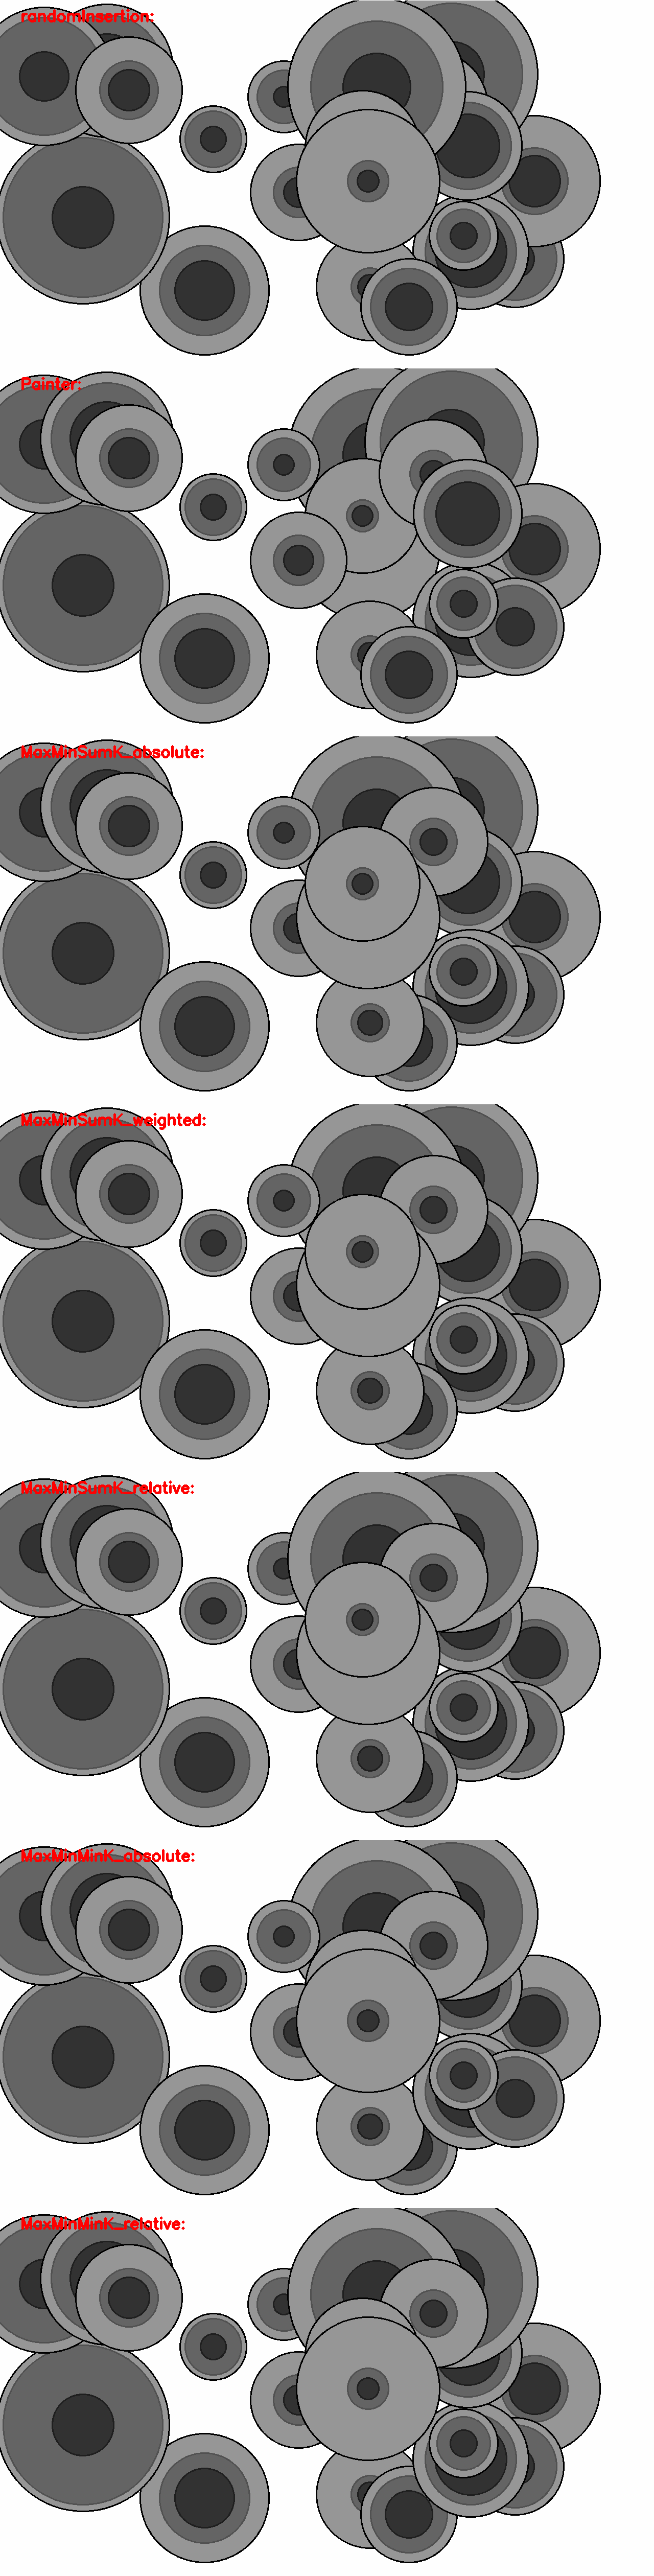
\includegraphics[width=\textwidth,height=0.7\textheight,keepaspectratio]{assets/cost_functions.png}
%\end{figure}

\begin{figure}[htp]
  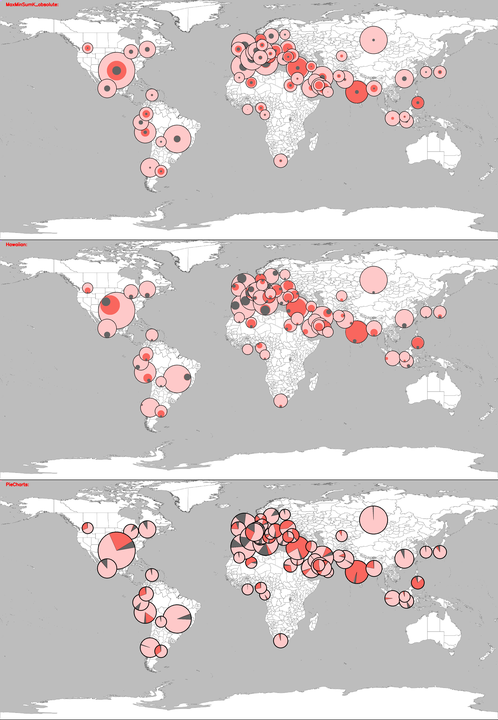
\includegraphics[width=\textwidth,height=\textheight,keepaspectratio]{assets/covid19_nested_discs.png}
\end{figure}

%\begin{figure}[htp]
%  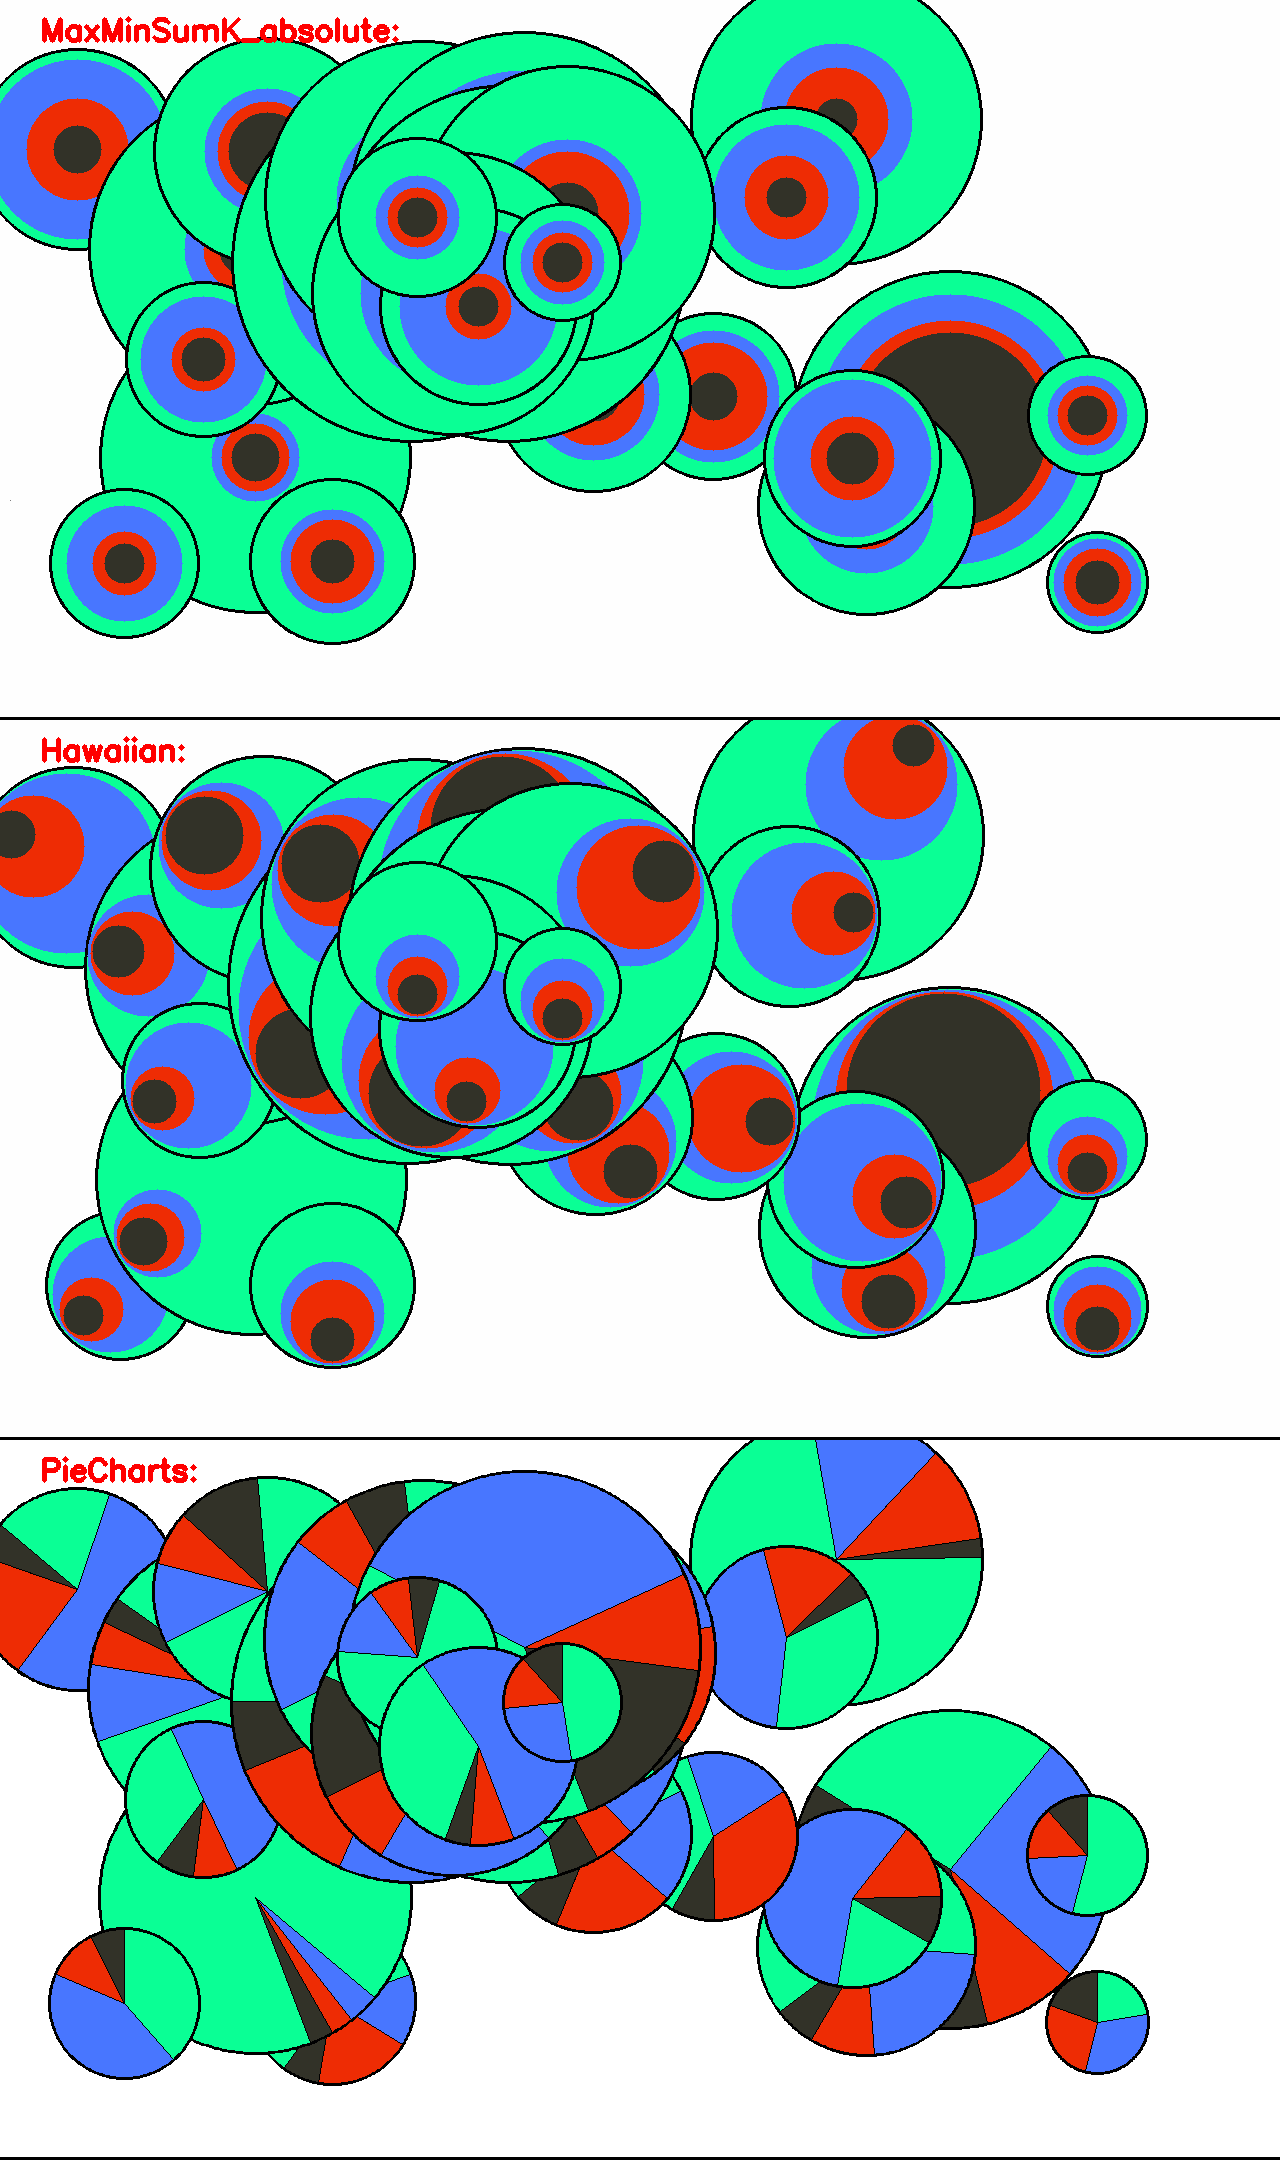
\includegraphics[width=\textwidth,height=\textheight,keepaspectratio]{assets/nested_discs_all.png}
%\end{figure}

\newpage

\begin{thebibliography}{999}

\bibitem [1] {tufte}Tufte, Edward R. "The visual display of quantitative information graphics press." Cheshire, Connecticut (1983).\\

\bibitem [2] {miller}Miller, Nancy, et al. "The need for metrics in visual information analysis." Proceedings of the 1997 workshop on New paradigms in information visualization and manipulation. 1997.\\

\bibitem [3] {brath}Brath, Richard. "Metrics for effective information visualization." Proceedings of VIZ'97: Visualization Conference, Information Visualization Symposium and Parallel Rendering Symposium. IEEE, 1997.\\

\bibitem [4] {tatu}Tatu, Andrada, et al. "Visual quality metrics and human perception: an initial study on 2D projections of large multidimensional data." Proceedings of the International Conference on Advanced Visual Interfaces. 2010.\\

\bibitem [5] {urribarri}Urribarri, D. K., \& Castro, S. M. (2016). Prediction of data visibility in two-dimensional scatterplots. Information Visualization, 16(2), 113–125. doi:10.1177/1473871616638892\\

\bibitem [6] {coeurjolly}Coeurjolly, D., Miguet, S., \& Tougne, L. (2004). 2D and 3D visibility in diskrete geometry: an application to diskrete geodesic paths. Pattern Recognition Letters, 25(5), 561–570. doi:10.1016/j.patrec.2003.12.002\\

\bibitem [7] {Yang}Yang-Pelaez J and Flowers WC. Information content
measures of visual displays. In: Proceedings of the IEEE symposium on information vizualization 2000 (INFOVIS’00), 2000, pp. 99–103. Washington, DC: IEEE Computer Society.\\

\bibitem [8] {cabello}Sergio Cabello, Herman Haverkort, Marc van Kreveld, Bettina Speckmann. Algorithmic Aspects of Proportional Symbol Maps. In: Algorithmica (2010) 58: 543–565. Published with open access at Springerlink.com.%



\end{thebibliography}

  ----------------------
\end{document}
% ----------------------

\begin{enumerate}
  \item Information content covered by the data,
  \item information content of the data in the visualization,
  \item information capacity of a visualization,
  \item topological information content.
\end{enumerate}

\begin{enumerate}
  \item Random inseration
  \item Painter
  \item MaxMinSumK/absolute - Sum of visible circumference/hull
  \item MaxMinSumK/weighted - weighted such that big circles/glyphs not dominate
  \item MaxMinSumK/relative - Sum of relative circumference/hull
  \item MaxMinMinK/absolute - MaxMin of minimal visible circumference/hull of each circle/glyph
  \item MaxMinMinK/relative
\end{enumerate}

Let $D$ be a finite set and for $d \in D$ and $S \subseteq D$ the function $ \phi(d, S) \mapsto \Re_{\geq 0} $ with the property, that for every $d \in D$ $S' \subseteq S => \phi(d, S') \geq \phi(d, S)$.

Let the stacking-order $\pi: \{1,...,n\} \mapsto D$ be bijective.

The algorithm

\begin{verbatim}
ALG(finite set D) {
  x := argmax_{d \in D} \phi(d, D \setminus {d})
  return [x, ALG(D \setminus {x})]
}
\end{verbatim}

returns a stacking-order, which maximizes $min_{d \in D} \phi(d, \{d\ \in D | d' > d\})$.

\unsure{Roland: shouldn't it be 'minimizes'?}

\begin{proof}
  Given an optimal stacking-order $s$ and output of ALG $s^*$ .

  \begin{enumerate}
    \item case: $s=s^*$. Done.
    \item case: $s \neq s^*$. $s \neq s^*$ implies, that there is a lowest $k \in N$, such that $s(k) \neq s^*(k)$. Let $s(k) = d_k$ and $s^* = d^*_k$. Hence, $k^* = s^{-1}(s^*(k)) = s^{-1}(d^*_k)$ is the index of $d^*_k$ with respect to $s$. It follows $k<k^*$.

          We modify $s$ such, that at point in time\unsure{Roland: point in 'time'? It's an order so it would be 'at position' as far as I see.}, we insert disk $d^*_k$ and shift all others towards the end. Let this new stacking-order be $s'$.
          \inlineinfo{Roland: What end, small or large end?}

          Comparing $s$ and $s'$, we find that $s'$ selects all disks later. That means, that all $\phi$-values are at least bigger.

          Now $d^*_k$ is chosen in $s'$, as well as in $s^*$ at position $k$.\unsure{Roland: Argumentiere hier mit Position. Das macht mEn mehr Sinn. Warte auf Eure Kommentare.} As $d^*_k$ was chosen by $s^*$, $d^*_k$ has to maxmize $\phi$. Therefore, it is bigger or equal to $d_k$, as $s$ and $s^*$ are identical except at position $k$.

  \end{enumerate}
\end{proof}

\begin{remark}
  $\phi$ may be the visible glyph boundary, the visible glyph boundary, the visible surface or the distance of...\unsure{Roland: Proof stops.}
\end{remark}


\begin{enumerate}
  \item Rotation
  \item Physics/Heuristics based approaches
\end{enumerate}

\begin{figure}[htp]
  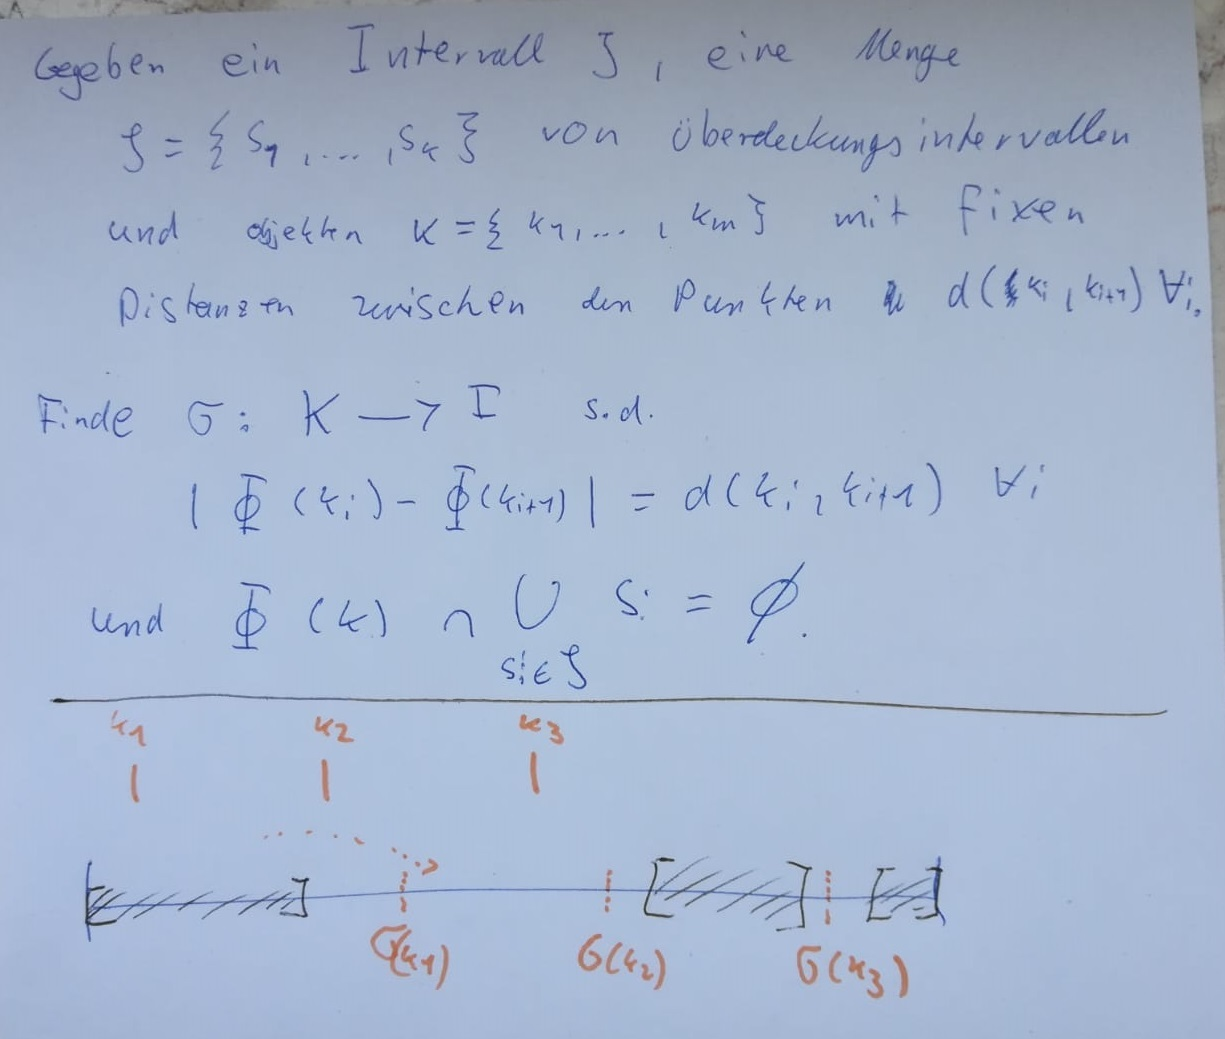
\includegraphics[width=\textwidth,height=\textheight,keepaspectratio]{assets/trennlinienproblem.jpg}
  \caption{Trennlinienproblem}
\end{figure}




% code from http://rosettacode.org/wiki/Fibonacci_sequence#Python
\begin{lstlisting}[label={list:first},caption=Sample Python code -- Fibonacci sequence calculated analytically.]
from math import *

# define function
def analytic_fibonacci(n):
  sqrt_5 = sqrt(5);
  p = (1 + sqrt_5) / 2;
  q = 1/p;
  return int( (p**n + q**n) / sqrt_5 + 0.5 )

# define range
for i in range(1,31):
  print analytic_fibonacci(i)
\end{lstlisting}

Following Listing~\ref{list:first}\ldots{}

Tufte proposed to measure quality based on the amount of consumed ink and purpose of the ink. He stated that the majority of the used ink in a graph must represent information about the data. Most recently Tatu et al. showed "that quality measures can simulate the selection of best views by human beings." and also compares a set of promising and established measures. In the motivated usecase, especially scatterplots using glyphs like circles or disks are of major interest, because of their advantages when plotting multidimensional data [Tatu et al.].\\

In a first step, following the common depiction, we consider circles as glyph. Further, we assume that the data $\mathcal{D}$ is finite and three-dimensional. We map two dimensions to the location $(x_i, y_i)$ and the remaining one dimension of our data set to the radius $r_i$ of a circle $C_i$, i.e., $ (x_i, y_i, r_i) \in \mathcal{D} \subset \mathbb{R}^3$. Moreover, we ignore transparency and other means to circumvent the occlusion of circles overlaying each other.\\

As already mentioned in the Motivation we want to maximize visibility of the data. Urribari et al define visibility as
%
\begin{equation} \label{eq1}
  \begin{split}
    visiblity & = 1 - occlusion \\
    & = f(data(set), visualization \, parameters)\\
  \end{split}
\end{equation}
%
with $occlusion$ being defined as [Tatu et al.]:
%
\begin{equation}
  occlusion = { \text{no. of data points completely occluded } \over \text{total no. of data points}}\\
\end{equation}

Using this simple definition it is possible to formulate two equivalent cost functions already now:
%
\begin{equation} \label{eq3}
  \begin{split}
    \min\limits_{\text{vis. par.}} & \; occlusion\\
    \max\limits_{\text{vis. par.}} & \; visiblity\\
  \end{split}
\end{equation}
%
We focus on visiblity for now. When using circles as glyphs, we can split the visibilty in two components:
%
\begin{equation} \label{eq3}
  \begin{split}
    U_i = & \delta C_i \, \setminus \bigcup_{D} C_j\\
    A_i = & \, C_i \; \setminus \bigcup_{D} C_j\\
  \end{split}
\end{equation}
%
and sum over the visible circumferences and areas
%
\begin{equation} \label{eq3}
  \begin{split}
    U_{occlusion} & = \sum_i U_i\\
    A_{occlusion} & = \sum_i A_i\\
  \end{split}
\end{equation}
%
which already hints toward potential cost functions.\\

Here many variations and specific options are thinkable. Like considering (1) relative circumference to circle area, (2) relative area to circumference, etc.
